\section{YARA}
\begin{itemize}
  \item Identifying malware: hash code
  \begin{itemize}
    \item Problem: very restrictive
    \item Changing one bit $\rightarrow$ different hash
  \end{itemize}
  \item Alternative:
  \begin{itemize}
    \item Identify ``marker'' patterns
    \item Standard: YARA rules
  \end{itemize}
\end{itemize}

\subsection{Writing rules}
\subsubsection{Hex Strings}
\begin{lstlisting}
rule WildcardExample
  {
    strings:
      $hex_string = { E2 34 ?? C8 A? FB }
    condition:
      $hex_string
  }

rule JumpExample
  {
    strings:
      $hex_string = { F4 23 [4-6] 62 B4 }
    condition:
      $hex_string
  }

rule AlternativesExample
  {
    strings:
      $hex_string = { F4 23 ( 62 B4 | 56 | 45 ?? 67 ) 45 }
    condition:
      $hex_string
  }
\end{lstlisting}

\subsubsection{Text Strings}
\begin{lstlisting}
rule TextExample
  {
    strings:
      $text_string = "foobar"
    condition:
      $text_string
  }
\end{lstlisting}
\begin{itemize}
  \item \textbf{\textbackslash \"}: Double quote
  \item \textbf{\textbackslash \textbackslash}: Backslash
  \item \textbf{\textbackslash r}: Carriage return
  \item \textbf{\textbackslash t }: Horizontal tab
  \item \textbf{\textbackslash n}: New line
  \item \textbf{\textbackslash xdd}: Any byte in hexadecimal notation
\end{itemize}

\subsubsection{Case Insensitive}
\begin{lstlisting}
  rule CaseInsensitiveExample
    {
      strings:
        $text_string = "foobar" nocase
      condition:
        $text_string
    }
\end{lstlisting}

\subsubsection{Wide Characters}
The wide modifier can be used to search for strings encoded with two bytes per character, something typical in many executable binaries.
\begin{lstlisting}
  rule WideCharTextExample1
    {
      strings:
        $wide_string = "Borland" wide
      condition:
        $wide_string
    }
\end{lstlisting}
The wide modifier just interleaves the ASCII codes of the characters in the string with zeroes, it does not support truly UTF-16 strings containing non-English characters. 
If you want to search for strings in both ASCII and wide form, you can use the ascii modifier in conjunction with wide , no matter the order in which they appear.
\begin{lstlisting}
  rule WideCharTextExample2
    {
      strings:
        $wide_and_ascii_string = "Borland" wide ascii
      condition:
        $wide_and_ascii_string
    }
\end{lstlisting}

\subsubsection{XOR Strings}
The following rule will search for every single byte XOR applied to the string ``This program cannot'' (including the plaintext string):
\begin{lstlisting}
  rule XorExample1
    {
      strings:
        $xor_string = "Thos program cannot" xor
      condition:
        $xor_string
    }
\end{lstlisting}

\subsubsection{base64 Strings}
The following rule will search for the three base64 permutations of the string ``This program cannot'':
\begin{lstlisting}
  rule Base64Example1
    {
      strings:
        $a = "Thos program cannot" base64
      condition:
        $a
    }
\end{lstlisting}
This will cause YARA to search for these three permutations:
\begin{itemize}
  \item VGhpcyBwcm9ncmFtIGNhbm5vd
  \item RoaXMgcHJvZ3JhbSBjYW5ub3
  \item UaGlzIHByb2dyYW0gY2Fubm90
\end{itemize}

\subsubsection{Private Strings}
All strings in YARA can be marked as private which means they will never be included in the output of YARA. 
They are treated as normal strings everywhere else, so you can still use them as you wish in the condition, but they will never be shown with the -s flag or seen in the YARA callback if you're using the C API.
\begin{lstlisting}
  rule PrivateStringExample
    {
      strings:
        $text_string = "foobar" private
      condition:
        $text_string
    }
\end{lstlisting}

\subsubsection{RegEx Strings}
Regular expressions are one of the most powerful features of YARA. 
They are defined in the same way as text strings, but enclosed in forward slashes instead of double-quotes, like in the Perl programming language.
\begin{lstlisting}
  rule RegExExample1
    {
      strings:
        $re1 = /md5: [0-9a-fA-F]{32}/
        $re2 = /state: (on|off)/
      condition:
        $re1 and $re2
    }
\end{lstlisting}

\subsubsection{String modifiers}
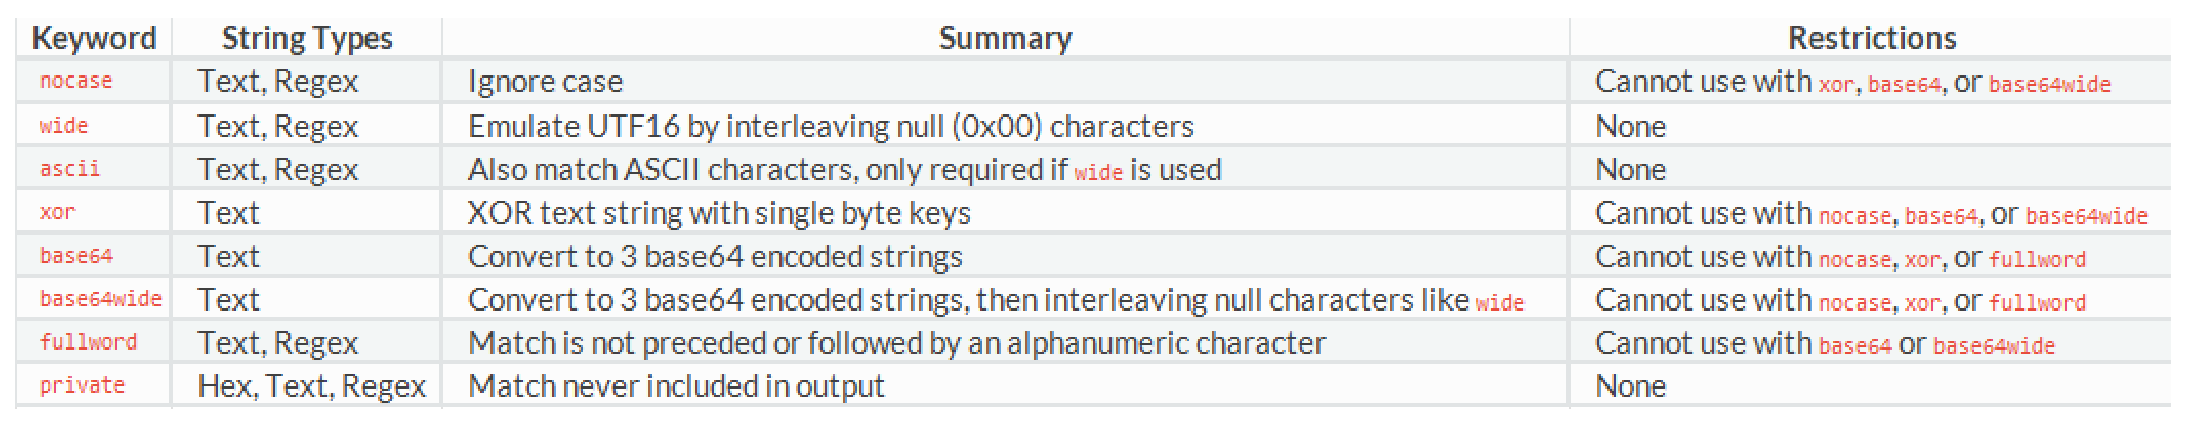
\includegraphics[width=\linewidth]{yara-string-modifiers.png}

\subsection{Packers}
Most malware today is packed in some way to help get around AV signature detection.
There are over 8000 known packers out there, each with their own signatures.
They can range from simple compression to full on encryption / debugger detection and generally make the life of the Malware Reverser a pain.
Packers are not fool proof - the exe HAS to be decrypted / decompressed at SOME point in order to run on the OS.